\documentclass[border=14pt]{standalone}
\usepackage[utf8]{inputenc}
\usepackage[T1]{fontenc}
\usepackage{circuitikz}
\usepackage{amsmath}
\usepackage{amssymb}
\usetikzlibrary{positioning,backgrounds,fit,calc}
\ctikzset{bipoles/length=1.1cm}

\begin{document}
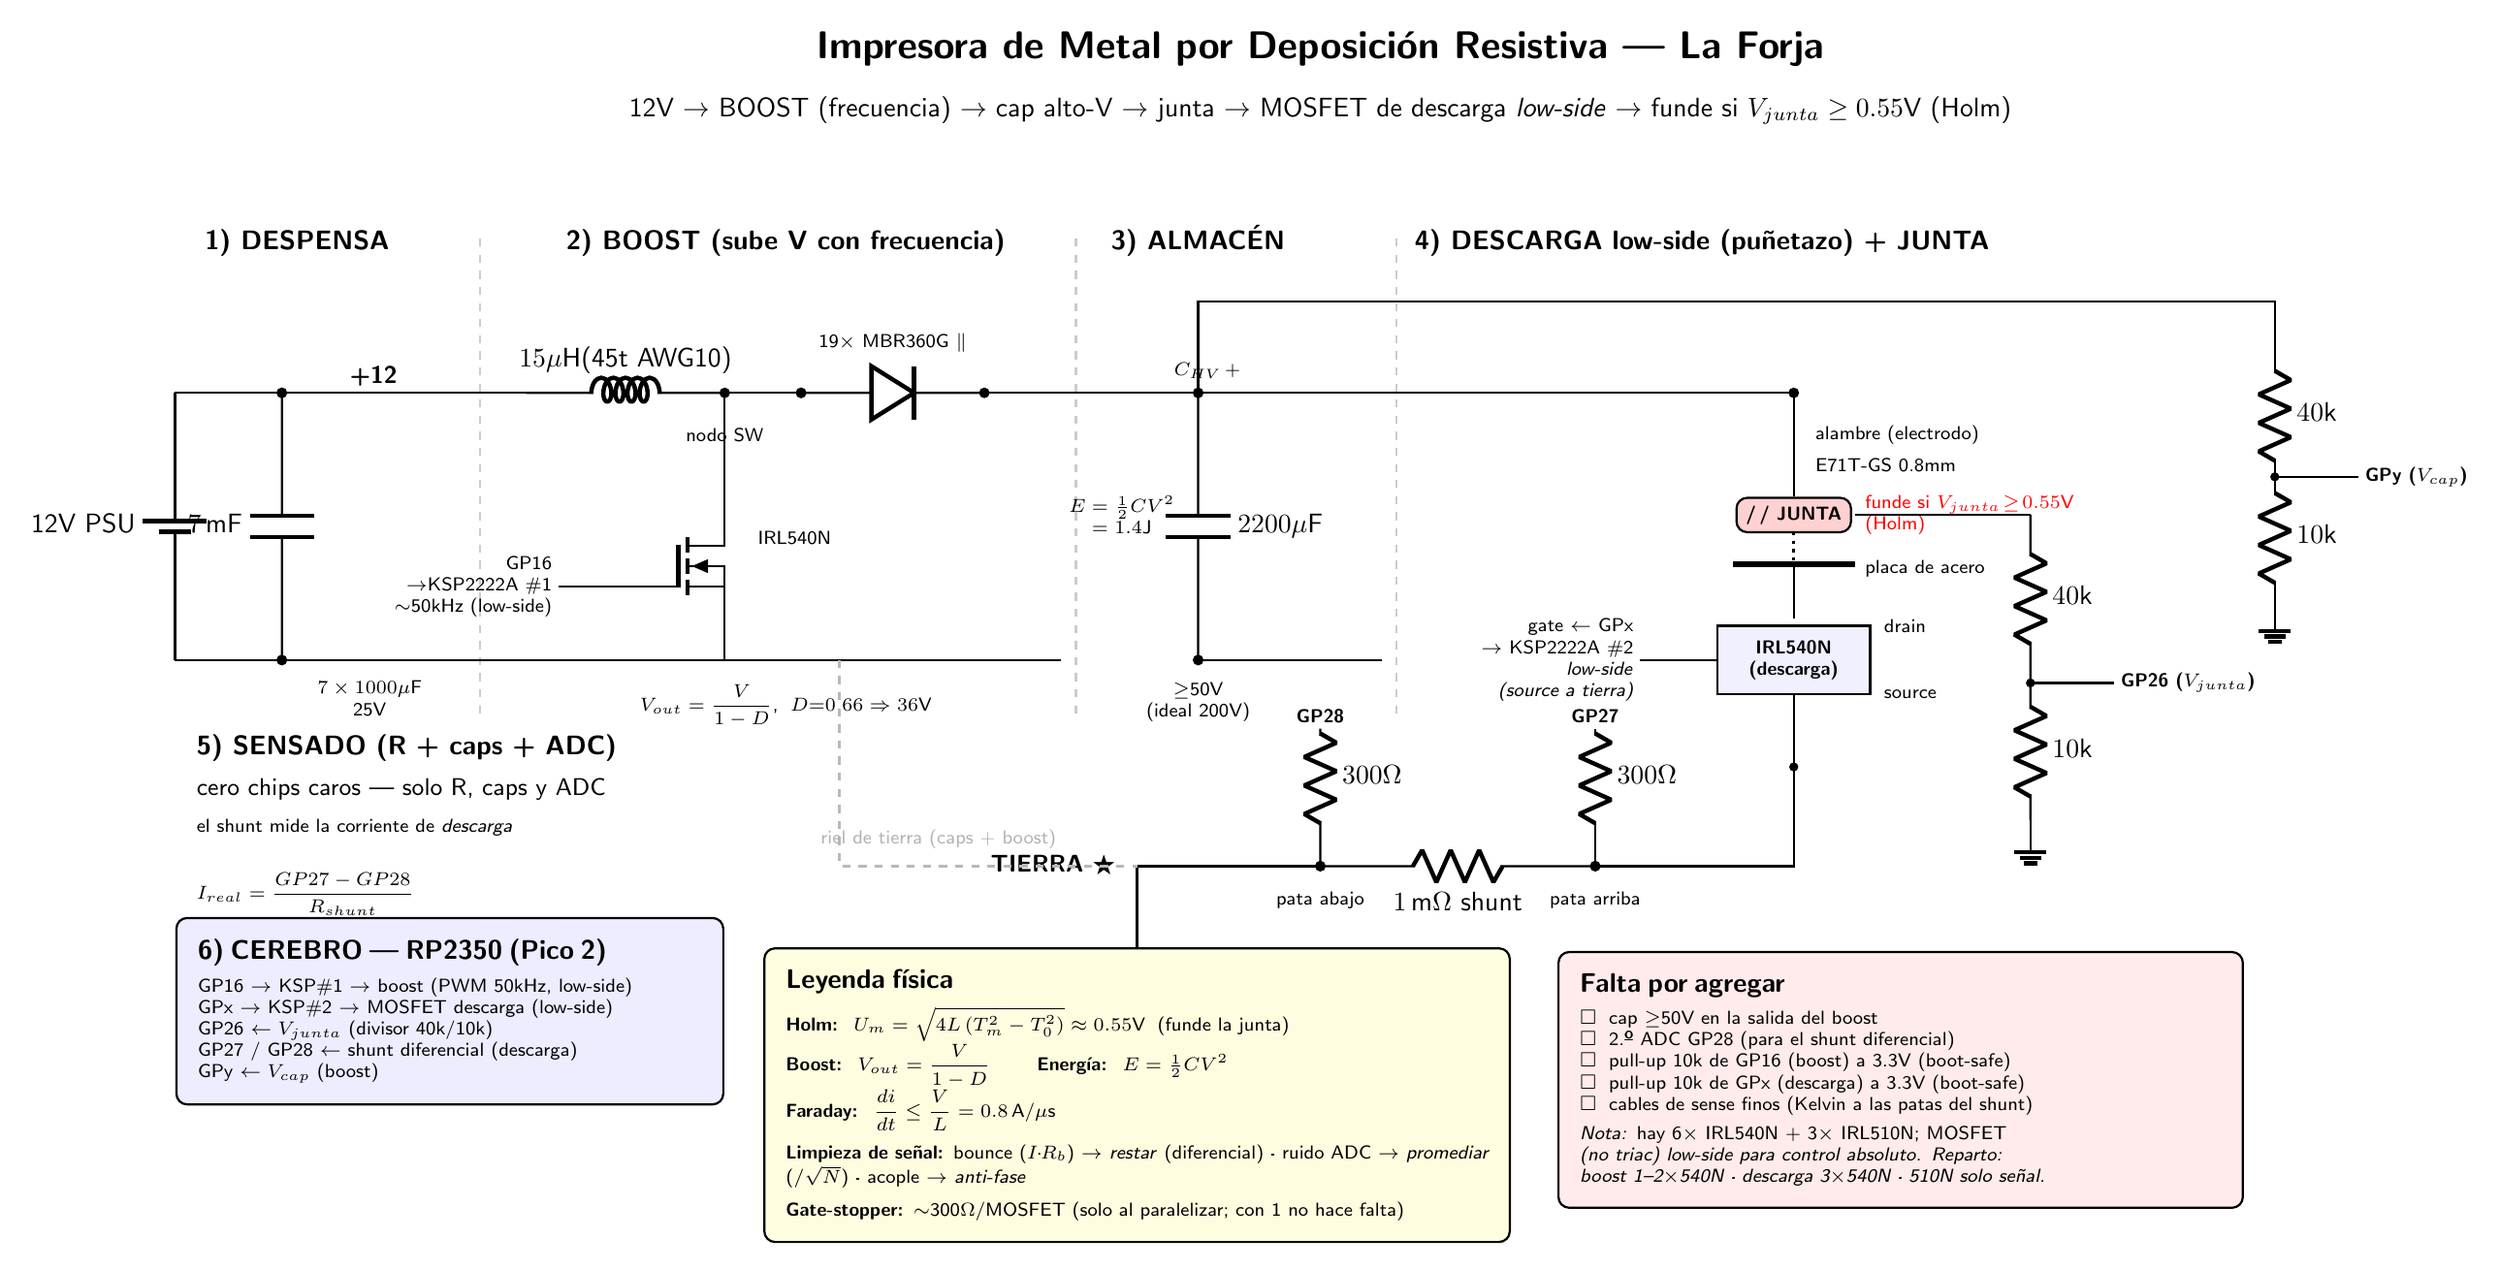
\begin{tikzpicture}[font=\sffamily,line width=0.8pt,
    every node/.style={inner sep=2pt}]

% ============================================================
%  TITULO
% ============================================================
\node[font=\sffamily\Large\bfseries] at (15,15)
  {Impresora de Metal por Deposición Resistiva — La Forja};
\node[font=\sffamily\normalsize] at (15,14.2)
  {12V $\rightarrow$ BOOST (frecuencia) $\rightarrow$ cap alto-V $\rightarrow$ junta $\rightarrow$ MOSFET de descarga \emph{low-side} $\rightarrow$ funde si $V_{junta}\ge 0.55$V (Holm)};

% Rieles de referencia (alto = +V, bajo = tierra)
% +V riel a y=10.5 ; tierra a y=7.0

% ============================================================
%  ETAPA 1 — DESPENSA  (x: 0 .. 4)
% ============================================================
\node[font=\sffamily\bfseries,anchor=south] at (1.6,12.2) {1) DESPENSA};

% fuente 12V
\draw (0,7.0) to[battery1,l=12V PSU,invert] (0,10.5);
% riel + arriba
\draw (0,10.5) -- (1.4,10.5);
% riel tierra abajo
\draw (0,7.0)  -- (1.4,7.0);
% banco de caps
\draw (1.4,10.5) to[C,l_=$7\,$mF,*-*] (1.4,7.0);
\node[font=\sffamily\scriptsize,align=center] at (2.55,6.5) {$7\times1000\mu$F\\25V};
% rieles que salen hacia el boost
\draw (1.4,10.5) -- (3.8,10.5) node[midway,above,font=\sffamily\small\bfseries]{+12};
\draw (1.4,7.0)  -- (3.8,7.0);

% separador punteado
\draw[gray!40,dashed] (4.0,6.3) -- (4.0,12.6);

% ============================================================
%  ETAPA 2 — BOOST  (x: 4 .. 12)
% ============================================================
\node[font=\sffamily\bfseries,anchor=south] at (8.0,12.2) {2) BOOST (sube V con frecuencia)};

% choque del +12 al nodo SW (riel superior)
\draw (3.8,10.5) -- (4.6,10.5);
\draw (4.6,10.5) to[L,l=$15\mu$H\\(45t AWG10)] (7.2,10.5) coordinate(SW);

% etiqueta nodo SW
\node[font=\sffamily\scriptsize,fill=white,inner sep=1pt] at (7.2,9.95) {nodo SW};
\node[circle,fill,inner sep=1.4pt] at (SW) {};

% rama del MOSFET: nodo SW -> drain -> source -> tierra
\draw (SW) -- (7.2,9.0);
\node[nigfete,anchor=D,rotate=0] (Q) at (7.2,9.0) {};
\draw (Q.G) -- ++(-1.2,0) node[left,font=\sffamily\scriptsize,align=right]{GP16\\$\rightarrow$KSP2222A \#1\\$\sim$50kHz (low-side)};
\draw (Q.S) -- (7.2,7.0);
\node[font=\sffamily\scriptsize,anchor=west] at (7.55,8.6) {IRL540N};

% banco de 19 diodos del nodo SW al cap HV
\draw (SW) -- (8.2,10.5);
\draw (8.2,10.5) to[D,*-] (10.6,10.5) coordinate(BOUT);
\node[font=\sffamily\scriptsize,align=center] at (9.4,11.15) {19$\times$ MBR360G $\parallel$};

% nodo de salida del boost
\node[circle,fill,inner sep=1.4pt] at (BOUT) {};
\draw (BOUT) -- (11.6,10.5);

% tierra del boost
\draw (3.8,7.0) -- (11.6,7.0);

% formula del boost
\node[font=\sffamily\scriptsize,align=center] at (8.0,6.4)
  {$V_{out}=\dfrac{V}{1-D}$,\; $D{=}0.66\Rightarrow 36$V};

% separador punteado
\draw[gray!40,dashed] (11.8,6.3) -- (11.8,12.6);

% ============================================================
%  ETAPA 3 — ALMACEN  (x: 12 .. 16)
% ============================================================
\node[font=\sffamily\bfseries,anchor=south] at (13.4,12.2) {3) ALMACÉN};

% cap HV
\draw (11.6,10.5) -- (13.4,10.5);
\node[font=\sffamily\scriptsize,anchor=south west] at (13.0,10.6) {$C_{HV}$\,+};
\draw (13.4,10.5) to[C,l=$2200\mu$F,*-*] (13.4,7.0);
\node[font=\sffamily\scriptsize,align=center] at (13.4,6.45) {$\ge$50V\\(ideal 200V)};
% energia almacenada (a la izquierda del cap, hueco libre entre boost y cap)
\node[font=\sffamily\scriptsize,align=center] at (12.4,8.9)
  {$E=\tfrac12 CV^2$\\$=1.4$J};

% riel + que sale hacia la descarga (el alambre cuelga de aquí)
\draw (13.4,10.5) -- (15.8,10.5);
% el riel de tierra (caps + boost source) NO pasa por el shunt:
% va DIRECTO a la tierra estrella (solo la descarga se mide en el shunt)
\draw (13.4,7.0)  -- (15.8,7.0);

% separador punteado
\draw[gray!40,dashed] (16.0,6.3) -- (16.0,12.6);

% ============================================================
%  ETAPA 4 — DESCARGA LOW-SIDE + JUNTA  (x: 16 .. 24)
% ============================================================
\node[font=\sffamily\bfseries,anchor=south] at (20.0,12.2) {4) DESCARGA \emph{low-side} (puñetazo) + JUNTA};

% el alambre cuelga DIRECTO del riel C_HV+ (sin MOSFET en el lado alto)
\draw (15.8,10.5) -- (21.2,10.5);
\node[circle,fill,inner sep=1.4pt] at (21.2,10.5) {};

% alambre / electrodo vertical (baja del riel +)
\draw (21.2,10.5) -- (21.2,9.6);
\node[font=\sffamily\scriptsize,anchor=west] at (21.4,9.95) {alambre (electrodo)};
\node[font=\sffamily\scriptsize,anchor=west] at (21.4,9.55) {E71T-GS 0.8mm};

% junta (zona roja)
\draw (21.2,9.6) -- (21.2,9.15);
\node[draw,fill=red!18,rounded corners,minimum width=1.5cm,minimum height=0.45cm,
      font=\sffamily\scriptsize\bfseries] (JU) at (21.2,8.9) {/\,/ JUNTA};
\node[font=\sffamily\scriptsize,red,anchor=west,align=left] at (22.05,8.9)
      {funde si $V_{junta}\!\ge\!0.55$V\\(Holm)};
\draw[dotted,line width=1.1pt] (21.2,8.67) -- (21.2,8.25);

% placa de acero
\draw[line width=2.2pt] (20.4,8.25) -- (22.0,8.25);
\node[font=\sffamily\scriptsize,anchor=west] at (22.05,8.2) {placa de acero};

% --- MOSFET de descarga LOW-SIDE: drain (arriba, a la placa) / source (abajo, al shunt) ---
\draw (21.2,8.25) -- (21.2,7.55);   % placa -> drain
\node[draw,minimum width=2.0cm,minimum height=0.9cm,fill=blue!6,
      font=\sffamily\scriptsize\bfseries,align=center] (QD) at (21.2,7.0)
      {IRL540N\\(descarga)};
\node[font=\sffamily\scriptsize,anchor=west] at (22.3,7.45) {drain};
\node[font=\sffamily\scriptsize,anchor=west] at (22.3,6.55) {source};
% gate a la IZQUIERDA, hacia el driver KSP #2 (low-side, sin opto)
\draw (QD.west) -- ++(-1.0,0)
      node[left,font=\sffamily\scriptsize,align=right]{gate $\leftarrow$ GPx\\$\rightarrow$ KSP2222A \#2\\\textit{low-side}\\\textit{(source a tierra)}};
% source baja hacia el shunt
\draw (21.2,6.55) -- (21.2,5.6);
\node[circle,fill,inner sep=1.2pt] at (21.2,5.6) {};

% ============================================================
%  ETAPA 5 — SENSADO  (debajo de la etapa 4: mide la DESCARGA)
% ============================================================
% Titulo en hueco libre, FAR LEFT
\node[font=\sffamily\bfseries,anchor=west] at (0.2,5.85)
  {5) SENSADO (R + caps + ADC)};
\node[font=\sffamily\small,anchor=west] at (0.2,5.3)
  {cero chips caros — solo R, caps y ADC};
\node[font=\sffamily\scriptsize,anchor=west] at (0.2,4.8)
  {el shunt mide la corriente de \emph{descarga}};

% --- shunt en el camino del SOURCE del MOSFET de descarga a tierra ---
% source baja a la pata-arriba (x=18.6), shunt horizontal, pata-abajo = tierra estrella
\draw (21.2,5.6) -- (21.2,4.3) -- (18.6,4.3) coordinate(SHA);
\node[circle,fill,inner sep=1.2pt] at (SHA) {};
\draw (SHA) to[R,l=$1\,$m$\Omega$ shunt,*-*] (15.0,4.3) coordinate(STAR);
\node[font=\sffamily\scriptsize,anchor=north] at (18.6,4.05) {pata arriba};
\node[font=\sffamily\scriptsize,anchor=north] at (15.0,4.05) {pata abajo};

% tierra estrella: aquí confluye el riel de tierra (caps + boost) DIRECTO
\draw (STAR) -- (12.6,4.3);
\draw (12.6,4.3) -- (12.6,3.4) node[ground]{};
\node[font=\sffamily\small\bfseries,anchor=east] at (12.4,4.3) {TIERRA $\bigstar$};
% el riel de tierra (y=7.0, caps+boost source) baja a la estrella SIN pasar por el shunt
\draw[gray!55,dashed] (8.7,7.0) |- (12.6,4.3);
\node[font=\sffamily\scriptsize,gray!60,anchor=south] at (10.0,4.45){riel de tierra (caps + boost)};

% sense diferencial: 300 ohm a GP27 (pata arriba) y GP28 (pata abajo)
\draw (18.6,4.3) -- (18.6,4.8) to[R,l_=$300\Omega$] (18.6,6.1)
      node[above,font=\sffamily\scriptsize\bfseries]{GP27};
\draw (15.0,4.3) -- (15.0,4.8) to[R,l_=$300\Omega$] (15.0,6.1)
      node[above,font=\sffamily\scriptsize\bfseries]{GP28};

% formula del sensado diferencial (hueco propio a la izquierda del shunt)
\node[font=\sffamily\scriptsize,align=left,anchor=west] at (0.2,3.6)
  {$I_{real}=\dfrac{GP27-GP28}{R_{shunt}}$\\[3pt](diferencial $\Rightarrow$ el ground bounce,\\común, se cancela)};

% divisor V_junta -> GP26  (lado derecho, columna propia x=24.3)
\draw (22.0,8.9) -- (24.3,8.9);
\draw (24.3,8.9) to[R,l=$40$k] (24.3,6.7);
\node[circle,fill,inner sep=1.2pt] at (24.3,6.7) {};
\draw (24.3,6.7) -- (25.4,6.7) node[right,font=\sffamily\scriptsize\bfseries]{GP26 ($V_{junta}$)};
\draw (24.3,6.7) to[R,l=$10$k] (24.3,4.9) node[ground]{};

% divisor V_cap -> GPy
% tap del nodo superior del cap HV (x=13.4,y=10.5); riel alto libre (y=11.7)
% hasta la columna far-right x=27.5 (clara), y baja el divisor 40k/10k
\node[circle,fill,inner sep=1.2pt] at (13.4,10.5) {};
\draw (13.4,10.5) -- (13.4,11.7) -- (27.5,11.7) -- (27.5,11.0);
\draw (27.5,11.0) to[R,l=$40$k] (27.5,9.4);
\node[circle,fill,inner sep=1.2pt] at (27.5,9.4) {};
\draw (27.5,9.4) -- (28.6,9.4) node[right,font=\sffamily\scriptsize\bfseries]{GPy ($V_{cap}$)};
\draw (27.5,9.4) to[R,l=$10$k] (27.5,7.8) node[ground]{};

% ============================================================
%  ETAPA 6 — CEREBRO RP2350  (caja azul, abajo-izquierda)
% ============================================================
\node[draw,rounded corners,fill=blue!7,align=left,font=\sffamily\scriptsize,
      text width=6.6cm,inner sep=8pt] (rpi) at (3.6,2.4) {
  \textbf{\normalsize 6) CEREBRO — RP2350 (Pico 2)}\\[4pt]
  GP16 $\rightarrow$ KSP\#1 $\rightarrow$ boost (PWM 50kHz, low-side)\\
  GPx $\rightarrow$ KSP\#2 $\rightarrow$ MOSFET descarga (low-side)\\
  GP26 $\leftarrow V_{junta}$ (divisor 40k/10k)\\
  GP27 / GP28 $\leftarrow$ shunt diferencial (descarga)\\
  GPy $\leftarrow V_{cap}$ (boost)};

% ============================================================
%  CAJA — LEYENDA FISICA
% ============================================================
\node[draw,rounded corners,fill=yellow!12,align=left,font=\sffamily\scriptsize,
      text width=9.2cm,inner sep=8pt] (fis) at (12.6,1.3) {
  \textbf{\normalsize Leyenda física}\\[4pt]
  \textbf{Holm:}\; $U_m=\sqrt{4L\,(T_m^2-T_0^2)}\approx 0.55$V \;(funde la junta)\\
  \textbf{Boost:}\; $V_{out}=\dfrac{V}{1-D}$ \qquad
  \textbf{Energía:}\; $E=\tfrac12 CV^2$\\
  \textbf{Faraday:}\; $\dfrac{di}{dt}\le\dfrac{V}{L}=0.8$\,A/$\mu$s\\[4pt]
  \textbf{Limpieza de señal:} bounce ($I\!\cdot\!R_b$) $\rightarrow$ \emph{restar} (diferencial) ·
  ruido ADC $\rightarrow$ \emph{promediar} ($/\sqrt{N}$) · acople $\rightarrow$ \emph{anti-fase}\\[4pt]
  \textbf{Gate-stopper:} $\sim$300$\Omega$/MOSFET (solo al paralelizar; con 1 no hace falta)};

% ============================================================
%  CAJA — FALTA POR AGREGAR
% ============================================================
\node[draw,rounded corners,fill=red!8,align=left,font=\sffamily\scriptsize,
      text width=8.4cm,inner sep=8pt] (falta) at (22.6,1.5) {
  \textbf{\normalsize Falta por agregar}\\[4pt]
  $\square$\; cap $\ge$50V en la salida del boost\\
  $\square$\; 2.º ADC GP28 (para el shunt diferencial)\\
  $\square$\; pull-up 10k de GP16 (boost) a 3.3V (boot-safe)\\
  $\square$\; pull-up 10k de GPx (descarga) a 3.3V (boot-safe)\\
  $\square$\; cables de sense finos (Kelvin a las patas del shunt)\\[3pt]
  \textit{Nota:} hay 6$\times$ IRL540N + 3$\times$ IRL510N; MOSFET\\
  \textit{(no triac) low-side para control absoluto. Reparto:}\\
  \textit{boost 1--2$\times$540N · descarga 3$\times$540N · 510N solo señal.}};

\end{tikzpicture}
\end{document}
